\documentclass[a4paper,11pt]{article}
\usepackage{amssymb}
\usepackage[polish]{babel}
\usepackage[utf8]{inputenc}
\usepackage[T1]{fontenc}
\usepackage{array}
\usepackage{graphicx}
\usepackage{anysize}
\usepackage{enumerate}
\usepackage{times}
\usepackage{geometry}
\usepackage{amsthm}
\usepackage{pgfplots}
\usepackage{tabularx}
\usepackage{sidecap}
\usepackage{wrapfig}
\usepackage[format=hang,font=small,labelfont=bf]{caption}


\usepackage[intlimits]{amsmath}
\marginsize{3cm}{3cm}{1.5cm}{1.5cm}
\sloppy

\begin{document}
\begin{table}[ht]
\centering
\hspace*{-1cm}
\begin{tabular}{lllllll}
\cline{1-6}
\multicolumn{1}{|c|}{\begin{tabular}[c]{@{}c@{}}EAIiIB\\ Informatyka\end{tabular}}              & \multicolumn{2}{l|}{\begin{tabular}[c]{@{}l@{}}Aleksander Lisiecki\\ Natalia Materek\end{tabular}}                                                                                                & \multicolumn{1}{c|}{\begin{tabular}[c]{@{}c@{}}Rok\\ II\end{tabular}}          & \multicolumn{1}{c|}{\begin{tabular}[c]{@{}c@{}}Grupa\\ 2\end{tabular}}            & \multicolumn{1}{c|}{\begin{tabular}[c]{@{}c@{}}Zespół\\ 6\end{tabular}}      &  \\ \cline{1-6}
\multicolumn{1}{|c|}{\begin{tabular}[c]{@{}c@{}}Pracownia\\ FIZYCZNA\\ WFiIS AGH\end{tabular}} & \multicolumn{4}{l|}{\begin{tabular}[c]{@{}l@{}}Temat:\\ \textbf{\textit{Mostek Wheastone'a}} \end{tabular}}                                                                                                                                                                                                                                            & \multicolumn{1}{c|}{\begin{tabular}[c]{@{}c@{}}Nr ćwiczenia:\\ 32\end{tabular}} &  \\ \cline{1-6}
\multicolumn{1}{|l|}{\begin{tabular}[c]{@{}c@{}}Data wykonania:\\ 18.12.2016\end{tabular}}      & \multicolumn{1}{c|}{\begin{tabular}[c]{@{}c@{}}Data oddania:\\ 21.12.2016\end{tabular}} & \multicolumn{1}{l|}{\begin{tabular}[c]{@{}l@{}}Zwrot do poprawki:\\ \phantom{data poprawki}\end{tabular}} & \multicolumn{1}{l|}{\begin{tabular}[c]{@{}l@{}}Data oddania:\\  \phantom{data oddania}\end{tabular}} & \multicolumn{1}{l|}{\begin{tabular}[c]{@{}l@{}}Data zaliczenia:\\  \phantom{data zaliczenia}\end{tabular}} & \multicolumn{1}{l|}{\begin{tabular}[c]{@{}l@{}}OCENA:\\ \phantom{ocena}\end{tabular}}       &  \\ \cline{1-6}
                                                                                                
\end{tabular}
\end{table}

\begin{center}
\begin{LARGE}
\textbf{Ćwiczenie nr 32: Mostek Wheastone'a}
\end{LARGE}
\end{center}

\section{Cel ćwiczenia}
\indent Celem ćwiczenia było zapoznanie z zasadą działania mostka Wheatstone’a w oparciu o prądowe i napięciowe prawo Kirchoffa służące do opisu złożonych obwodów elektrycznych oraz metody pomiaru nieznanych oporów oraz ich połączeń szeregowych i równoległych zgodnie z prawem Ohma.

\section{Wstęp teoretyczny}
\begin{wrapfigure}{l}{0.4\textwidth}
\label{rys:1}
\vspace*{-0.5cm}
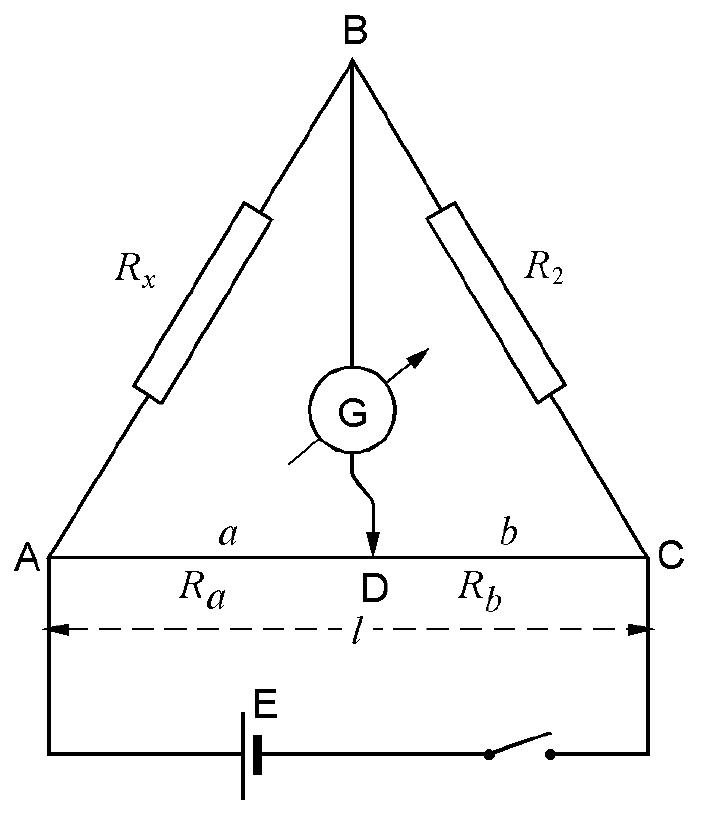
\includegraphics[width=0.4\textwidth]{./schemat}
\end{wrapfigure}
\indent Mostek Wheatstone’a jest jednym z klasycznych sposobów dokładnego pomiaru nieznanego oporu elektrycznego. Załóżmy, że mamy nieznany opór $R_x$, znane opory $R_a$, $R_b$ oraz regulowaną opornicę dekadową o oporze $R_2$. Zestawiamy następujący obwód: do szeregowego połączenia oporów $R_x$, $R_2$ przyłączamy równolegle połączenie szeregowe $R_a$, $R_b$. Węzły pomiędzy wspomnianymi parami oporów łączymy galwanometrem. Po przyłożeniu do układu różnicy potencjałów możemy regulować $R_2$ tak, aby galwanometr wskazywał 0, czyli brak różnicy potencjałów, a co za tym idzie i brak przepływu prądu między odpowiednimi węzłami. Wtedy z praw Ohma i Kirchhoffa możemy wyprowadzić następujące wzory: 
\begin{equation}
\label{wzor:1}
I_a\cdot R_a=I_x\cdot R_x
\end{equation}

\begin{equation}
\label{wzor:2}
I_b\cdot R_b=I_d\cdot R_2
\end{equation}
gdzie
\begin{description}
\item [$I_{a}$] natężenie prądu na odcinku A[$A$]
\item [$I_{b}$] natężenie prądu na odcinku B[$A$]
\item [$R_{a}$] opór na odcinku A[$\Omega$]
\item [$R_{b}$] opór na odcinku B[$\Omega$]
\item [$R_{x}$] opór nieznany[$\Omega$]
\item [$R_{2}$] opór regulowanej opornicy dekadowej[$\Omega$]
\end{description}
\indent Ze wzorów {\ref{wzor:1}} i {\ref{wzor:2}} wynika równość spadków napięć na odpowiednich oporach oraz równość odpowiednich natężeń prądów, czyli:
$$I_a=I_b$$
$$I_x=I_d$$

gdzie 
\begin{description}
\item[$I_{d}$] natężenie [$A$]
\item[$I_{x}$] natężenie [$A$]

\end{description}
\indent Stąd można wyprowadzić wyrażenie na $R_x$:
\begin{equation}
\label{wzor:3}
R_x=R_a\frac{I_a}{I_x}=R_a\frac{I_b}{I_d}=R_2\frac{R_a}{R_b}
\end{equation}

Ponieważ $R_a$ i $R_b$ są oporami odcinków tego samego jednorodnego drutu, ich wielkości są proporcjonalne do długości:
\begin{equation}
\label{wzor:4}
\frac{R_a}{R_b}=\dfrac{a}{b}=\dfrac{a}{l-a}
\end{equation}

gdzie 
\begin{description}
\item[$a$] długość odcinka AD [$m$]
\item[$b$] długość odcinka DC [$m$]
\end{description}
Ostatecznie otrzymujemy, że:

\begin{equation}
\label{wzor:5}
R_x=R_2\dfrac{a}{l-a}
\end{equation}

gdzie 
\begin{description}
\item[$R_{2}$] opór wzorcowy [$\Omega$]
\item [$a$] zmierzona długość na listwie [$m$]
\end{description}
\indent Dokładność pomiaru mostkiem Wheatstone’a z drutem oporowym zależy przede wszystkim od błędu wyznaczenia odległości $a$. Aby pomiar był najdokładniejszy należy tak dobrać opór $R_2$, aby stan równowagi mostka można było uzyskać w przybliżeniu w połowie długości drutu oporowego.

\section{Układ pomiarowy}
Układ mostka Wheatstone’a pokazany został na rysunku {\ref{rys:1}}. W~skład obwodu wchodzą:
\begin{itemize}
\item Listwa z drutem oporowym, zaopatrzona w podziałkę milimetrową i kontakt ślizgowy umożliwiający zmiany długości odcinków $a$ i $b$.
\item  Opornica dekadowa
\item  Zestaw oporników oznaczony symbolem $R_x$, umieszczony na płytce z pleksiglasu.
\item Mikroamperomierz $G$ jako wskaźnik zerowania mostka. Jego czułość można regulować.
\item Zasilacz.
\end{itemize}

\section{Przebieg doświadczenia}
\indent Przy przeprowadzaniu eksperymentu skorzystano z układu pomiarowego, którego schemat przedstawia rysunek {\ref{rys:1}}. 
\indent Pomiędzy punktami $A$ i $C$ znajduje się listwa z  drutem oporowym o znanej długości. $R_2$ jest opornikiem wzorcowym o regulowanej wartości oporu, a $R_x$ nieznanym oporem, którego wartość chcemy wyznaczyć. Zrównoważenie mostka polega na takim ustawieniu punktu $D$, aby dla zadanej wartości $R_2$ przez galwanometr nie płynął prąd.
\begin{itemize}
\item Ustawienie oporu wzorcowego na opornicy dekadowej.
\item Zrównoważenie mostka przez ustawienie kontaktu ślizgowego tak, aby dla zadanej wartości oporu przez galwanometr nie płynął prąd.
\item Odczytanie wartości $a$ na której zatrzymano kontakt ślizgowy.
\item Czynności od 1 do 3 powtórzono dziesięciokrotnie dla oporników $R_{x1}$, $R_{x2}$ oraz tych samych oporników połączonych szeregowo i równolegle.
\item Wyznaczenie wartości nieznanych oporów na podstawie wzoru {\ref{wzor:5}}.
\item Wyznaczenie $R_{\text{śr}}$ jako sumy arytmetycznej oporów z poszczególnych dziesięciu prób.
\end{itemize}

\section{Wyniki pomiarów}

\begin{table}[h!]
\caption{Opornik $R_{x1}$}
\begin{tabular}{|l|c|c|c|c|c|c|c|c|c|c|}\hline
\label{table1}
Opór wzorcowy & 102 & 60 & 50 & 40 & 30 & 20 & 15 & 95 & 70 & 25 \\ \hline
$a [mm]$ & 121 & 184 & 226 & 262 & 321 & 425 & 477 & 131 & 173 & 379 \\ \hline
$R_{x_{1}} [\Omega]$ &  & 13,53 & & & & & & & \\ \hline
\end{tabular}

\begin{tabular}{|l|l|}\hline
$ \overline{R}_{x_{1}} \approx$ ... & $u(\overline{R}_{x_{1}}) \approx$ ...  \\ \hline
\end{tabular}
\end{table}

\begin{table}[h!]
\caption{Opornik $R_{x2}$}
\begin{tabular}{|l|c|c|c|c|c|c|c|c|c|c|}\hline
\label{table1}
Opór wzorcowy & 25 & 35 & 30 & 20 & 15 & 10 & 5 & 8 & 12 & 18 \\ \hline
$a [mm]$ & 453 & 362 & 383 & 504 & 550 & 669 & 746 & 671 & 607 & 494 \\ \hline
$R_{x_{1}} [\Omega]$ &  & 19,86 & & & & & & & \\ \hline
\end{tabular}

\begin{tabular}{|l|l|}\hline
$ \overline{R}_{x_{2}} \approx$ ... & $u(\overline{R}_{x_{2}}) \approx$ ...  \\ \hline
\end{tabular}
\end{table}

\begin{table}[h!]
\caption{Połączenie szeregowe $R_{x1}$ i $R_{x2}$}
\begin{tabular}{|l|c|c|c|c|c|c|c|c|c|c|}\hline
\label{table1}
Opór wzorcowy & 20 & 18 & 15 & 12 & 22 & 25 & 30 & 35 & 40 & 45 \\ \hline
$a [mm]$ & 642 & 617 & 688 & 703 & 588 & 562 & 530 & 478 & 445 & 422 \\ \hline
$R_{x_{1}} [\Omega]$ &  & 28,00 & & & & & & & \\ \hline
\end{tabular}

\begin{tabular}{|l|l|}\hline
$ \overline{R} \approx$ ... & $u(\overline{R}) \approx$ ...  \\ \hline
\end{tabular}
\end{table}


\begin{table}[h!]
\caption{Połączenie równoległe $R_{x1}$ i $R_{x2}$}
\begin{tabular}{|l|c|c|c|c|c|c|c|c|c|c|}\hline
\label{table1}
Opór wzorcowy & 12 & 15 & 18 & 20 & 23 & 27 & 10 & 8 & 6 & 3 \\ \hline
$a [mm]$ & 444 & 383 & 321 & 309 & 290 & 246 & 468 & 522 & 549 & 716 \\ \hline
$R_{x_{1}} [\Omega]$ & 9,583 & 9,311 & 8,510 & 8,944 & 9,394 & 8,809 & 8,797 & 8,736 & 7,304 & 7,563\\ \hline
\end{tabular}

\begin{tabular}{|l|l|}\hline
$ \overline{R} \approx$ ... & $u(\overline{R}) \approx$ ...  \\ \hline
\end{tabular}
\end{table}

\section{Opracowanie wyników pomiarów}
\indent Aby obliczyć opór nieznany $R_x$ korzystamy z powyższego wzoru {\ref{wzor:5}}
Listwa ma długość 100 [$cm$].

\indent Niepewność typu A oporu $R_x$ wyznaczamy z następującego wzoru:
\begin{equation}
u(R_x) = \sqrt{\frac{\sum \left( R_i - \overline{R}_x \right)^2 }{n(n-1)}}
\end{equation}
gdzie 
\begin{description}
\item [$u(R_{x})$] niepewność pomiaru oporu [$\Omega$]
\item [$R_{i}$] opór z i -tej próby [$\Omega$]
\item [$\overline{R}_x$] wartość średnia oporu [$\Omega$]
\item [$n$] liczba prób
\end{description}

Po podstawieniu odpowiednich wartości otrzymujemy:
$$
u(R_{x_{1}}) = \sqrt{\frac{(... - ...)^2 + \cdots (... - ...)^2  }{10(10-1)}}\approx ... ~\Omega
$$

$$
u(R_{x_{2}}) = \sqrt{\frac{(.. - ...)^2 + \cdots (... - ...)^2  }{10(10-1)}} \approx ... ~\Omega
$$

$$
u(R_{z_s}) = \sqrt{\frac{(... - ...)^2 + \cdots (... - ....)^2  }{10(10-1)}} \approx ... ~\Omega
$$

$$
u(R_{z_r}) = \sqrt{\frac{(... - ...)^2 + \cdots (... - ...)^2  }{10(10-1)}} \approx ... ~\Omega
$$

gdzie
\begin{description}
\item [$u(R_x1)$] niepewność pomiaru oporu dla opornika $R_{x1}$ [$\Omega$]
\item [$u(R_x2)$] niepewność pomiaru oporu dla opornika $R_{x2}$ [$\Omega$]
\item [$u(R_{z_s})$] niepewność pomiaru oporu dla oporników $R_{x1}$ i $R_{x2}$ połączonych szeregowo[$\Omega$]
\item [$u(R_{z_r})$] niepewność pomiaru oporu dla oporników $R_{x1}$ i $R_{x2}$ połączonych równolegle[$\Omega$]
\end{description}

\subsection{Połączenie szeregowe}
\indent Wartość oporu przy połączeniu szeregowym można też obliczyć na podstawie wzoru na opór zastępczy oraz wyznaczonych wartości $R_{x_1}$ i  $R_{x_2}$

$$
R_{obl} = R_{x_1} + R_{x_2} \approx ... ~\Omega
$$
\indent Niepewność dla wartości wyliczanych ze wzorów na opór zastępczy w obwodzie z połączeniem szeregowym wyznaczamy z prawa przenoszenia niepewności i opisujemy wzorem:
\begin{center}
\begin{align*}
u(R_{obl}) &= \sqrt{\left( \frac{\delta R_{z_{s}} }{\delta R_{x_1}}  \right)^2 u(R_{x_1})^2  +\left( \frac{\delta R_{z_{s}} }{\delta R_{x_2}}  \right)^2  u(R_{x_2})^2  } \\
& = \sqrt{u(R_{x_1})^2 + u(R_{x_2})^2} \\
&\approx ... ~\Omega
\end{align*}
\end{center}
gdzie 
\begin{description}
\item [$u(R_{\text{obl}})$] niepewność oporu ... [$\Omega$]
\end{description}

\subsection{Połączenie równoległe}
\indent Wartość oporu przy połączeniu równoległym można też obliczyć na podstawie wzoru na opór zastępczy oraz wyznaczonych wartości $R_{x_1}$ i  $R_{x_2}$

$$ 
R_{z_r} = \frac{ R_{x_1} R_{x_2}}{ R_{x_1} + R_{x_2}} \approx ...~\Omega
$$
\begin{center}
\begin{align*}
u(R_{obl}) &= \sqrt{\left( \frac{\delta R_{z_r} }{\delta R_{x_1}}  \right)^2 u(R_{x_1})^2  +\left( \frac{\delta R_{z_r} }{\delta R_{x_2}}  \right)^2  u(R_{x_2})^2  }\\ 
& =  \sqrt{\left(  \frac{R_{x_1}}{R_{x_1} + R_{x_2}}\right)^4  u(R_{x_1})^2 + \left(\frac{R_{x_2}}{R_{x_1} + R_{x_2}}\right)^4  u(R_{x_2})^2}\\ 
&\approx  ...~\Omega
\end{align*}
\end{center}


\subsection{Porównanie wartości z pomiarów i wyznaczonych ze wzorów}
\begin{tabularx}{\textwidth}{XXX}
\hline
 & \textbf{Opory zmierzone}  & \textbf{Opory ze wzoru} \\ 
\hline \textbf{Połączenie szeregowe} & $... ~\Omega$ & $... ~\Omega$ \\ 
\hline \textbf{Połączenie równoległe} & $...~\Omega$& $...) ~\Omega$\\ 
\hline 
\end{tabularx} 
\section{Wnioski}
\begin{itemize} 
\item Opory wyznaczone w ćwiczeniu mają zbliżone wartości do obliczonych ze wzorów, jednak nie mieszczą się/mieszcza sie? w granicach niepewności pomiarowych (nawet w granicach niepewności rozszerzonej dla współczynnika rozszerzenia $k=2$.).
\item Błędy mogą wynikać ze złego odczytania wartości z amperomierza, bądź złego odczytania długości drutu, lub niedokładności urządzeń pomiarowych.
 
\end{itemize}

\end{document}